\section{\method}
\paragraph{実験に用いる装置}このレポート内すべての実験にはMathWorks\raisebox{2mm}{\tiny\textregistered}社の\matlab を用いて,\tblref{tbl:実験環境}の環境下で実験する.
\begin{table}[H]
    \caption{実験環境}
    \label{tbl:実験環境}
    \begin{tabularx}{\textwidth}{AR}
        \hline
        実験機                      & MacBook Air 2022 (Apple社)\texttt{MLY13J/A}    \\
        プロセッサ                    & Apple Silicon M2\ \  8コアCPU,8コアGPU            \\
        メモリ                      & 8GB                                           \\
        \multirow{2}{*}{\matlab} & R2023a - academic use (Update1 9.14.02239454) \\
                                 & 64-bit (maci64) March 30, 2023                \\
        \hline
    \end{tabularx}
\end{table}
また,このレポート内すべての実験では\matlab でプロットしたグラフを出力するための\texttt{exportgraphics}関数,画像を書き出すための\texttt{imwrite}関数を用いる(\srcref{src:グラフ・画像出力}).
\begin{lstlisting}[numbers={none},caption={グラフ・画像出力},label={src:グラフ・画像出力}]
exportgraphics(figurename,'path/figure_name.pdf','ContentType','vector');
imwrite(data,"path/figure_name.png");
\end{lstlisting}
\paragraph{\kadaiaa}
RGB色空間の画像を,緑チャネルだけを抜き出してグレイスケール画像を作成する.赤チャネル,青チャネルについても同様にグレイスケール画像を生成する.さらに,RGB画像の赤チャネルと青チャネルを入れ替えたカラー画像を作成する.
\texttt{imwrite}関数を用いて,画像の読み込む.読み込んだ画像はRGB色空間で保存されており,チャネル1にはR,チャネル2にはG,チャネル3にはBが保存されている.
グレイスケール画像を作成するには,各チャネルの画素値を,\eqref{equ:grayscale}の割合で画像を加算合成する.\mat{m}{n}の行列\texttt{A}に対して,\mat{1}{n}を取り出したければ,\verb|A(1,:)|と記述する.\verb|:|は,すべての要素を表す記号である.
赤チャネルと青チャネルを入れ替えるためには,赤チャネルの行列と青チャネルの行列を変数に保存し,それぞれ互いのチャネルに代入する.\scall{\kadaiaa}\sref{src:05_01}.
\paragraph{\kadaiab}
グレイスケール画像を生成する.緑チャネルは色の濃淡を多く含む.RGB色空間から色の濃淡を抽出したい場合は,緑(G)の成分を多く抽出するとよい.具体的な割合を,\eqref{equ:grayscale}に示す.ここではNTSC輝度信号を取り出す方法で行う.生成したグレイスケール画像に対して,画像の量子化数を変更することによる,画像の変化を確認する.量子化数は8Bit,4Bit,2Bit,1Bitの4種をテストする.量子化数1Bitの画像を2値画像という.
\begin{align}
    \textrm{Gray scale image} & = \textrm{Red}\times 30\% +\textrm{Green}\times 59\% +\textrm{Blue}\times 11\%\label{equ:grayscale}
\end{align}
\begin{wrapfigure}{r}[0mm]{.3\textwidth}
    \centering
    \vspace{-.7cm}
    \begin{lstlisting}[caption={\texttt{bitshift}関数},label={src:bitshift}]
img = bitshift(img, n);
    \end{lstlisting}
    \vspace{-.5cm}
\end{wrapfigure}
量子化数を変更するために,\texttt{bitshift}関数を用いる(\srcref{src:bitshift}).
この関数は,\texttt{img}を左に\texttt{n}ビットシフトする関数である.右シフトしたい場合は\texttt{n}を負の数で与える.
ある数値を1ビット右シフトするごとに,その数値は\(1/2\)される.
これを利用して,量子化数4Bitの場合は右に4Bitシフト,量子化数2Bitの場合は右に6Bitシフト,量子化数1Bitの場合は右に7Bitシフトする.
量子化数4Bitを例にあげる.仮に画素値が\texttt{255}(白)を持つ画素の場合,量子化数を4Bitにする,つまり4Bit右シフトすると,画素値は\texttt{15}になる.このままでは画素値の範囲が\(0\)から\(15\)となる.
この対策として,全体画素値と\(255/15\)の積を取ることで,画素値を\(0\)から\(255\)にスケーリングする.\scall{\kadaiab}\sref{src:05_02}.
\paragraph{\kadaiac}
各量子化数の画像に対して,その画像を階調反転させる.階調反転とは,白黒を反転させることである.量子化数による階調変換後の画像を比較する.
各量子化数ごとに階調反転する.階調反転を実現するためには,階調反転した画像を\texttt{double}型に変換したあと,\(-1\)との積をとり,\(255\)を足した後で\texttt{unit8}型に変換する\footnote{その画像の各画素値が\texttt{double}型であるとき,\texttt{imwrite}関数が,データを自動的にリスケールするため.}.\scall{\kadaiac}\sref{src:05_03}.

\begin{wrapfigure}{r}[0mm]{.3\textwidth}
    \centering
    \vspace{-.7cm}
    \begin{lstlisting}[caption={判定結果の格納},label={src:判定結果の格納}]
mat = [1 2 3; 4 5 6; 7 8 9];
bin = mat > 5;
% -- 結果 --
bin = [0 0 0; 0 0 1; 1 1 1];     
    \end{lstlisting}
    \vspace{-.5cm}
\end{wrapfigure}
\paragraph{\kadaiad}
閾値処理とは,とある値より大きい場合を白,その値未満を黒とし,2値画像を作成することである.この値を閾値という.
\matlab には,判定結果の真理値を行列に格納する機能がある.
\srcref{src:判定結果の格納}より,行列\texttt{mat}の各元が\(5\)より大きい箇所を\(1\),\(5\)以下のところを\(0\)とする行列\texttt{bin}を作成できる.この行列を真理行列と呼ぶ.
この機能を用いて,ある閾値に対して,閾値よりも大きければ\(1\)を戻し,閾値以下であれば\(0\)を戻す行列を作成する.画素値の範囲を\(0\)から\(255\)へするために,行列の各元と\(255\)の積をとる.今回は,閾値を\(64\),\(128\),\(192\)で実験する.\scall{\kadaiad}\sref{src:05_04}

\begin{wrapfigure}{r}[0mm]{.3\textwidth}
    \centering
    \vspace{-1cm}
    \begin{lstlisting}[caption={\texttt{sum}関数},label={src:sum関数}]
matA = [1 2 3];
s_matA = sum(matA); 
% -> 出力:6
matB = [1 2; 1 1; 1 1];
s_matB = sum(matB); 
% -> 出力:[3 4]
s_s_matB = sum(sum(matB)); 
% -> 出力:12
    \end{lstlisting}
    \vspace{-1cm}
\end{wrapfigure}
\paragraph{\kadaiae}
量子化数8Bitのグレイスケール画像のヒストグラムを作成する.画素値\((0,1,\dots ,255)\)の画素が何画素含まれているかのヒストグラムを作成する.
ヒストグラムを作成するために,この関数は行列の元を足し合わせる\texttt{sum}関数を用いる(\srcref{src:sum関数}).
各画素値\(0\)から\(255\)に対して,その画素値と等しい箇所を\(1\)とする真理行列を作成し,各元の和を\texttt{sum}関数を用いて算出する.
その結果は,ある画素値がいくつ画像に含まれているかを指す.
\paragraph{\kadaiaf}
被写体が写っている画像と,被写体を除いた背景だけが写っている画像の差分画像をとる.これを背景差分と呼ぶ.背景差分の後,閾値処理を行う.
固定カメラ\footnote{手での固定は,背景がズレる可能性があるので,カメラを固定して撮影した.}で撮影した写真を用いる.「背景と被写体が写っている画像\texttt{img\_sbj}」「背景のみの画像\texttt{img\_bg}」の2点を撮影した.背景差分画像は,\(\texttt{img\_sbj}-\texttt{img\_bg}\)で生成する.
生成した画像に対して,閾値を\(32\),\(64\),\(128\)で閾値処理する.閾値処理する前後での画像比較,閾値による比較する.\scall{\kadaiaf}\sref{src:05_06}.

\begin{wrapfigure}{r}[0mm]{.3\textwidth}
    \vspace{-1cm}
    \begin{lstlisting}[caption={白色ガウス雑音画像の生成},label={src:白色ガウス雑音画像の生成}]
% 画像サイズ : n x m
wgn = 10*randn(n, m);
wgn = uint8(wgn);
wgn_img = wgn + gimg;
    \end{lstlisting}
    \begin{lstlisting}[caption={インパルス雑音画像の生成},label={src:インパルス雑音画像の生成}]
% 画像サイズ : n x m
rnd = rand(n, m);
b = (rnd < 0.01);
w = (rnd > 0.99);
in_img(w) = 255;
in_img(b) = 0;
    \end{lstlisting}
    \vspace{-.5cm}
\end{wrapfigure}
\paragraph{画像フィルタ}
画像処理におけるフィルタは,画像ないに含まれる雑音を除去したり,特徴を抽出したりすることで欠陥検出をより円滑に行うための基本処理を指す\cite{画像フィルタ}.
\newcommand{\originimg}{\texttt{original\_img}}
\newcommand{\wgnimg}{\texttt{wgn\_img}}
\newcommand{\inimg}{\texttt{in\_img}}
今回の実験では,白色ガウス雑音とインパルス雑音を含んだ2つのテスト画像を用意する.グレイスケール元画像を\originimg とする.\par
白色ガウス雑音は,白色性を持つガウス雑音である.今回は,平均\(0\),標準偏差\(10\)としてガウス分布の乱数を発生させる.
このテスト画像を\wgnimg とする.
白色ガウス雑音の作成には\texttt{randn}関数を用い,生成した乱数と,標準偏差の積を取る.生成した乱数を\texttt{uint8}型に変換し,\originimg と和を取る(\srcref{src:白色ガウス雑音画像の生成}).
\(255\)を上回る,または\(0\)を下回る画素値を,\(0\)または\(255\)へ変換した画像を, \wgnimg とする.\par
インパルス雑音は,超短時間におこる高周波の雑音のことを指す.今回は,画像のランダムな画素を,白と黒で塗り替える.それぞれ全体画素の1\(\%\) の割合で作成する.
このテスト画像を\inimg とする.
インパルス雑音は,\texttt{rand}関数を用いて作成する.発生率を\(1\%\) にするため,乱数の\(0.01\)未満の画素を黒,乱数の\(0.99\)より大きい画素を白としてインパルスノイズを設計する(\srcref{src:インパルス雑音画像の生成}).
画像フィルタはいくつかの種類があり,画像雑音の除去やエッジの強調に用いられる.
\begin{enumerate}
    \item \textbf{平滑化フィルタ}
          \begin{itemize}
              \item 画像の各画素\(p\)に対して,\(n\)近傍と中央の画素値の平均や重み付け平均をとり,\(p\)の画素値とするフィルタ.
              \item 今回の実験では,各画素\(p\)に対して,\(3\times 3\),つまり8近傍と\(p\)の画素値の平均をとり,中央の画素値として定義する.
          \end{itemize}
    \item \textbf{メディアンフィルタ}
          \begin{itemize}
              \item 画像の各画素\(p\)に対して,\(n\)近傍と中央の画素値を昇順に整列し,その中央値を\(p\)の画素値とする.
              \item 今回の実験では,各画素\(p\)に対して,\(3\times 3\),つまり8近傍と\(p\)の画素値を昇順に整列する.その中央値を\(p\)の画素値として定義する.
          \end{itemize}
    \item \textbf{微分フィルタ}
          \begin{itemize}
              \item 微分フィルタは,境界線の強調や局所的な特徴の抽出するフィルタである.しかし,1次微分フィルタ,2次微分フィルタを用いると,画像の雑音も強調される.ここでPrewittフィルタとSobelフィルタを用いると,雑音がある画像でもうまく境界線を抽出できる\cite[p.87]{画像処理}.
                    \begin{itemize}
                        \item \textbf{Prewitt フィルタ}:隣り合う2画素の画素値を持ちいて3画素ずつをセットにして濃度の変化点を抽出するアルゴリズム\cite[p.87]{画像処理}.
                        \item \textbf{Sobel フィルタ}:画像の各ピクセルの周囲の画素との差を計算して,その差の大きさを使って,エッジを検出するアルゴリズム.
                    \end{itemize}
              \item 今回の実験では,\originimg に対して,Sobelフィルタを用いて縦微分,横微分,縦微分と横微分の加算合成した画像を作成する.
          \end{itemize}
    \item \textbf{Laplacianフィルタ}
          \begin{itemize}
              \item Laplacianフィルタは,微分フィルタ同様,境界線を見つけるために使われる方法である.
              \item 今回の実験では,\originimg に対して,8近傍Laplacianフィルタを適用し,閾値処理する.
          \end{itemize}
\end{enumerate}
\newpage
\begin{figure}[h]
    \centering
    \begin{minipage}[b]{.24\textwidth}
        \centering
        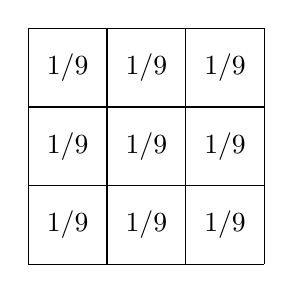
\begin{tikzpicture}
            \draw (0,0) grid (3,3);
            \foreach \u \v in {0.5/0.5,1.5/0.5,2.5/0.5,0.5/1.5,1.5/1.5,2.5/1.5,0.5/2.5,1.5/2.5,2.5/2.5}
            \node at (\u,\v) {\(1/9\)};
        \end{tikzpicture}
        \subcaption{平滑化フィルタ}
        \label{fig:平滑化フィルタ}
    \end{minipage}
    \begin{minipage}[b]{.24\textwidth}
        \centering
        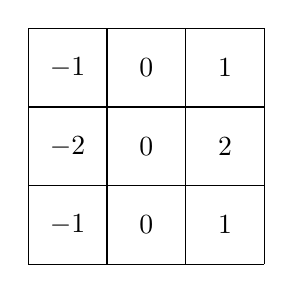
\begin{tikzpicture}
            \draw (0,0) grid (3,3);
            \foreach \u \v \w in {0.5/0.5/{\(-1\)},1.5/0.5/{\(0\)},2.5/0.5/{\(1\)},0.5/1.5/{\(-2\)},1.5/1.5/{\(0\)},2.5/1.5/{\(2\)},0.5/2.5/{\(-1\)},1.5/2.5/{\(0\)},2.5/2.5/{\(1\)}}
            \node at (\u,\v) {\w};
        \end{tikzpicture}
        \subcaption{Sobelフィルタ:横方向}
        \label{fig:Prewittフィルタ_横方向}
    \end{minipage}
    \begin{minipage}[b]{.24\textwidth}
        \centering
        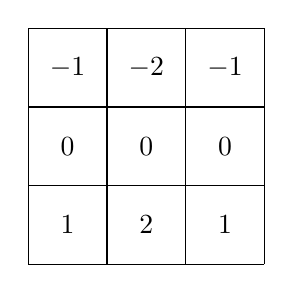
\begin{tikzpicture}
            \draw (0,0) grid (3,3);
            \foreach \u \v \w in {0.5/0.5/{\(1\)},1.5/0.5/{\(2\)},2.5/0.5/{\(1\)},0.5/1.5/{\(0\)},1.5/1.5/{\(0\)},2.5/1.5/{\(0\)},0.5/2.5/{\(-1\)},1.5/2.5/{\(-2\)},2.5/2.5/{\(-1\)}}
            \node at (\u,\v) {\w};
        \end{tikzpicture}
        \subcaption{Sobelフィルタ:縦方向}
        \label{fig:Prewittフィルタ_縦方向}
    \end{minipage}
    \begin{minipage}[b]{.24\textwidth}
        \centering
        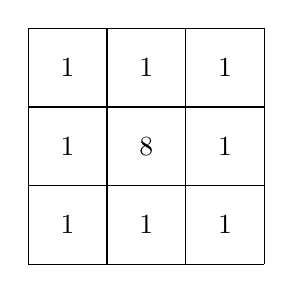
\begin{tikzpicture}
            \draw (0,0) grid (3,3);
            \foreach \u \v in {0.5/0.5,1.5/0.5,2.5/0.5,0.5/1.5,2.5/1.5,0.5/2.5,1.5/2.5,2.5/2.5}
            \node at (\u,\v) {\(1\)};
            \node at (1.5,1.5) {\(8\)};
        \end{tikzpicture}
        \subcaption{8近傍Laplacianフィルタ}
        \label{fig:Laplacianフィルタ}
    \end{minipage}
    \caption{\(3\times 3\)画像フィルタ}
\end{figure}
\paragraph{フィルタの適用}
平滑化フィルタ,微分フィルタ,Laplacianフィルタの適用は,\texttt{filter2}関数(\ \verb|filter2(filter, img)|\ )を用いる.
メディアンフィルタは,画像の\mat{i}{j}に対して\texttt{median}関数を用いてフィルタ処理する.メディアンフィルタを適用する際に,四方すべてに画素がない画素(\mat{1}{1}画素,\mat{m}{1}画素など)はフィルタ処理できないため,0パディング処理を行い,メディアンフィルタを適用する(\srcref{src:メディアンフィルタの適用}).
\begin{figure}[H]
    \centering
    \begin{minipage}[b]{.24\textwidth}
        \centering
        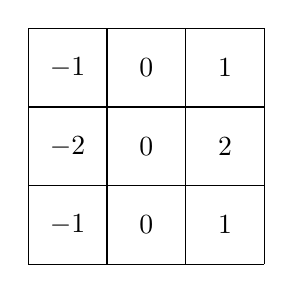
\begin{tikzpicture}[remember picture]
            \draw (0,0) grid (3,3);
            \foreach \u \v \w in {0.5/0.5/{\(-1\)},1.5/0.5/{\(0\)},2.5/0.5/{\(1\)},0.5/1.5/{\(-2\)},1.5/1.5/{\(0\)},2.5/1.5/{\(2\)},0.5/2.5/{\(-1\)},1.5/2.5/{\(0\)},2.5/2.5/{\(1\)}}
            \node at (\u,\v) {\w};
            \coordinate (aa) at (3,3);
            \coordinate (bb) at (3,0);
        \end{tikzpicture}
        \subcaption{Sobelフィルタ:縦方向}
    \end{minipage}
    \begin{minipage}[b]{.24\textwidth}
        \centering
        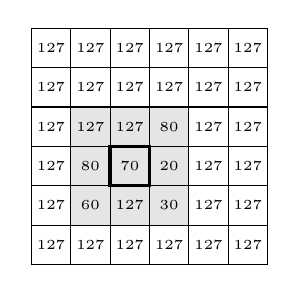
\begin{tikzpicture}[remember picture]
            \fill[gray!20] (0.5,0.5)rectangle(2,2);
            \draw[very thick] (1,1)rectangle(1.5,1.5);
            \draw[thin](0,0)grid[step=0.5](3,3);
            \foreach \u \z in {0.25/A, 0.75/B,1.25/C,1.75/D, 2.25/E, 2.75/F}{
                    \foreach \v \w in {0.25/A, 0.75/B,1.25/C,1.75/D, 2.25/E, 2.75/F}{
                            \coordinate (\z\w) at (\u,\v);
                        }
                }
            \foreach \u \v in {AA/127,AB/127,AC/127,AD/127,AE/127,AF/127, BA/127,BB/60,BC/80,BD/127,BE/127,BF/127, CA/127,CB/127,CC/70,CD/127,CE/127,CF/127, DA/127,DB/30,DC/20,DD/80,DE/127,DF/127, EA/127,EB/127,EC/127,ED/127,EE/127,EF/127, FA/127,FB/127,FC/127,FD/127,FE/127,FF/127}
            \node at (\u) {\tiny \v};
            \coordinate (ma) at (2,0.5);
            \coordinate (mb) at (2,2);
        \end{tikzpicture}
        \subcaption{フィルタを適用する画像}
    \end{minipage}
    \begin{minipage}[b]{.25\textwidth}
        {\scriptsize
            \begin{multline*}
                (-1\times 127)+(0\times 127)+(1\times 80)\\
                +(-2\times 80)+(0\times 70)+(2\times 20)\\
                +(-1\times 60)+(0\times 127)+(1\times 39)\\=-57
            \end{multline*}
        }
        \subcaption{フィルタ処理の演算}
    \end{minipage}
    \begin{minipage}[b]{.24\textwidth}
        \centering
        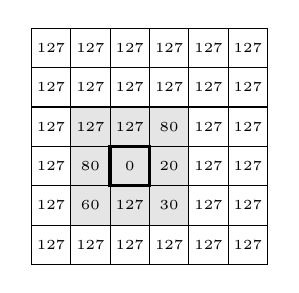
\begin{tikzpicture}
            \fill[gray!20] (0.5,0.5)rectangle(2,2);
            \draw[very thick] (1,1)rectangle(1.5,1.5);
            \draw[thin](0,0)grid[step=0.5](3,3);
            \foreach \u \z in {0.25/A, 0.75/B,1.25/C,1.75/D, 2.25/E, 2.75/F}{
                    \foreach \v \w in {0.25/A, 0.75/B,1.25/C,1.75/D, 2.25/E, 2.75/F}{
                            \coordinate (\z\w) at (\u,\v);
                        }
                }
            \foreach \u \v in {AA/127,AB/127,AC/127,AD/127,AE/127,AF/127, BA/127,BB/60,BC/80,BD/127,BE/127,BF/127, CA/127,CB/127,CC/0,CD/127,CE/127,CF/127, DA/127,DB/30,DC/20,DD/80,DE/127,DF/127, EA/127,EB/127,EC/127,ED/127,EE/127,EF/127, FA/127,FB/127,FC/127,FD/127,FE/127,FF/127}
            \node at (\u) {\tiny \v};
        \end{tikzpicture}
        \subcaption{フィルタ適用後の画素値}
    \end{minipage}
    \caption{フィルタ適用の実際}
\end{figure}
\begin{tikzpicture}[overlay,remember picture]
    \draw[line width=2pt, line cap=butt,draw=white](aa)--(mb);
    \draw[line width=2pt, line cap=butt,draw=white](bb)--(ma);
    \draw[dotted,thick](aa)--(mb);
    \draw[dotted,thick](bb)--(ma);
\end{tikzpicture}
\begin{lstlisting}[caption={メディアンフィルタの適用},label={src:メディアンフィルタの適用},frame={left}]
for h = 2:img_height % 画像行列 img の高さ
    for w = 2:img_width % 画像行列 img の横幅,median_filter は0パディング後のimg
        median_filter(h-1, w-1) = median(img(h-1:h+1,w-1:w+1),"all"); 
    end
end
\end{lstlisting}
\scall{ノイズ画像の生成とフィルタの適用}\sref{src:06_01} - \sref{src:06_04}.
\paragraph{色空間変換}
この実験では,RGB色空間から,HSV色空間へ変換する.RGB色空間は,赤(Red),緑(Green),青(Blue)の3チャネルで構成する.HSVは色相(Hue),彩度(Saturation),明度(Value)の3チャネルで構成する.
色相は,カラー ホイール上の色の位置に対応する,\(0\)から\(100\)の値,色相の量または中間からの逸脱,特定の色の赤,緑,青成分の中での最大値,いずれも\texttt{double}型で保存される\cite{rgb2hsv}.
読み込んだ画像はRGB色空間で保存される.この画像をHSV色空間に変換するためには,\texttt{rgb2hsv}関数を用いる.
出力された値と\(255\)の積を取り,HSV色空間で出力された画像を書き出す.
色相,彩度,明度それぞれのチャネルを抽出し,\matlab のアプリケーションを用いて,肌色要素のHSV成分を出力する(\sref{src:06_05_f}).
それぞれの値に合致した画素を,画素値\(255\),ほかの画素値を\(0\)とした画像を書き出す.同様な方法で,RGB色空間における肌色領域の抽出も行う(\sref{src:06_05_f2}).
\scall{\kadaibe}\sref{src:06_05},\sref{src:06_05_1}.
\paragraph{2次元フーリエ変換}
フーリエ変換は,任意の連続信号に対して各空間周波数成分が,どの程度含まれているかを示す変換である.音声などの1次元信号に対しては,離散1次元フーリエ変換を適用した.画像は2次元信号なので,2次元離散フーリエ変換し,空間周波数成分を取り出す.
出力されるスペクトルは,縦軸に\(y\)方向のスペクトル,横軸には\(x\)方向のスペクトル,輝度には成分の大きさが表現されている.
連続データにおいて,2次元フーリエ変換するためには,\eqref{equ:2次元フーリエ変換}を用いる.
また,離散データ,\mat{N}{M}の画像に対して,\mat{x}{y}画素の画素値を\(f(x,y)\),2次元フーリエ変換結果の\mat{u}{v}画素値を\(F(u,v)\)とすると,\(F(u,v)\)は\eqref{equ:2次元離散フーリエ変換}で求められる.
\begin{align}
    F(u,v) & =\int_{-\infty}^{\infty}\int_{-\infty}^{\infty}f(x,y)\exp\Big(-j2\pi\left(\frac{ux}{N}+\frac{vy}{N}\right)\Big)dxdy  & (j\textrm{は虚数単位})\label{equ:2次元フーリエ変換} \\
    F(u,v) & =\sum_{x=1}^{N}\sum_{y=1}^{M}f(x,y)\exp\Big(-j2\pi\left(\frac{ux}{N}+\frac{vy}{N}\right)\Big)\label{equ:2次元離散フーリエ変換}
\end{align}
ここで,\eqref{equ:直交成分}より,2次元フーリエ変換の直交成分\((u,v)=(0,0)\)の値\(F(0,0)\)は,全画素値の和である.
\begin{align}
    F(0,0) & = \sum_{x=1}^{N}\sum_{y=1}^{N}f(x,y)\label{equ:直交成分}
\end{align}
\matlab における高速2次元離散フーリエ変換\footnote{以降,高速2次元離散フーリエ変換を2次元フーリエ変換と記す.}は,\texttt{fft2}関数を用いる.出力したデータを整形するために,\texttt{fftshift}関数を用いる.
今回は,出力された空間周波数スペクトルを,パワースペクトル\footnote{パワーとは,各値を2乗したもの.}に変換して結果とする.一部の出力結果は,対数\footnote{パワースペクトルのデータを\texttt{power}とすると,\(\log(1+\texttt{power})\)で表現する.}をとって出力する.
出力結果のカラーマップをグレイスケールにする\texttt{colormap}関数,画像データの最大値を白,最小値を黒にスケーリングして出力する\texttt{imagesc}関数を用いる.\par
また,画像に対して高域通過フィルタを適用するには,パワースペクトルにフィルタを適用し,2次元逆フーリエ変換することでフィルタを適用した画像を得られる.
高域通過フィルタは,円形のフィルタを用いる.低周波数領域で,中心から半径\(50\textrm{pixel}\),\(100\textrm{pixel}\)以内の値を\(0\)にするとで,フィルタを適用する.
フィルタは,フーリエ変換後のデータと同じサイズの行列に対して,対象となる円領域を\(0\),ほかの領域を\(1\)とし,フィルタ\mat{m}{n}と,フーリエ変換後データ\mat{m}{n}との積を取ることで適用する.
ここで,\texttt{fft2}後の値は,虚数を含む複素数である.値は,複素数としての値で意味があり,パワースペクトルに対してフィルタを適用してはならない.逆フーリエ変換した複素数値を含むデータを\texttt{real}関数を用いて実数化し,画像として表示する.
\begin{lstlisting}[caption={2次元フーリエ変換と高域通過フィルタ},label={src:2次元フーリエ変換と高域通過フィルタ}]
% 画像データを data とする
fft_data = fftshift(fft2(data)); % 2次元フーリエ変換
power = abs(fft_data.^ 2); % 2次元フーリエ変換してパワースペクトルを生成する
log_power = log(1 + power); % 生成したパワースペクトルに対して対数を取る
% 高域通過フィルタを flt とする
fft_img = fft_data.*flt; % フィルタの適用
img = ifftshift(ifft2(fft_img)); % 2次元逆フーリエ変換
img = real(img); % 実数化
	\end{lstlisting}
\scall{2次元フーリエ変換}\sref{src:08_01}\ -\ \sref{src:08_04}.